\documentclass[12pt,a4paper]{article}
\usepackage[utf8]{inputenc}
\usepackage[T1]{fontenc}
\usepackage[italian]{babel}
\usepackage{geometry}
\usepackage{amsmath}
\usepackage{amssymb}
\usepackage{listings}
\usepackage{xcolor}
\usepackage{graphicx}
\usepackage{hyperref}
\usepackage{booktabs}
\usepackage{caption}
\usepackage{float}
\usepackage{parskip}
\usepackage{array}
\usepackage{tabularx}
\usepackage{tcolorbox}
\tcbuselibrary{listings,breakable,skins}
\usepackage{tikz}
\usetikzlibrary{arrows.meta, positioning, shapes.geometric, fit, calc}

\geometry{
  top=2.5cm, bottom=2.5cm,
  left=2.5cm, right=2.5cm
}

\definecolor{codebg}{RGB}{248,248,248}
\definecolor{keywordcolor}{RGB}{0,0,180}
\definecolor{commentcolor}{RGB}{0,128,0}
\definecolor{stringcolor}{RGB}{163,21,21}
\definecolor{codeframe}{RGB}{180,180,180}

\lstdefinestyle{python}{
  language=Python,
  basicstyle=\ttfamily\footnotesize,
  keywordstyle=\color{keywordcolor}\bfseries,
  commentstyle=\color{commentcolor}\itshape,
  stringstyle=\color{stringcolor},
  numberstyle=\tiny\color{gray},
  numbers=left,
  stepnumber=1,
  breaklines=true,
  breakatwhitespace=false,
  showstringspaces=false,
  tabsize=4,
  xleftmargin=1.5em,
  keepspaces=true,
  columns=flexible,
  frame=none,
  aboveskip=0pt,
  belowskip=0pt,
}
\lstset{style=python}

\hypersetup{
  colorlinks=true,
  linkcolor=blue!60!black,
  urlcolor=blue!60!black,
}

\newtcblisting{pylisting}[1][]{
  listing only,
  enhanced,
  colback=codebg,
  colframe=codeframe,
  coltitle=black,
  fonttitle=\small\itshape,
  attach boxed title to top left={yshift=-2mm, xshift=4mm},
  boxed title style={colback=codebg, colframe=codeframe, boxrule=0.5pt},
  boxrule=0.5pt,
  arc=2pt,
  left=4pt, right=4pt, top=8pt, bottom=4pt,
  listing options={style=python},
  before upper={\vspace{-2pt}},
  #1
}

\newcommand{\HRule}{\rule{\linewidth}{0.5mm}}

\begin{document}
\raggedbottom

% ============================================================
% FRONTESPIZIO
% ============================================================
\begin{titlepage}
  \centering
  \vspace*{1.5cm}

  {\Large\textbf{Università degli Studi di Torino}\\[0.3em]
  Corso di Laurea Magistrale in Informatica}

  \vspace{1cm}
  \HRule\\[0.4em]
  {\LARGE\textbf{Tecnologie del Linguaggio Naturale}}\\[0.3em]
  {\large Parte 2 -- Prof.\ Daniele Radicioni}\\[0.2em]
  \HRule

  \vspace{1.2cm}
  {\huge\textbf{Lab 8}}\\[0.5em]
  {\LARGE Word Clustering con Word2Vec}\\[0.4em]
  {\large Confronto tra testi musicali: anni 70 vs anni 2000}

  \vspace{2cm}

  {\large\textbf{Gruppo di lavoro:}}\\[0.8em]
  \begin{tabular}{ll}
    \toprule
    \textbf{Studente}    & \textbf{Matricola} \\
    \midrule
    Alessandro Olivero   & 915069  \\
    Samuele Iudice       & 1235245 \\
    Andrea Franco        & 1226739 \\
    \bottomrule
  \end{tabular}

  \vspace{1.5cm}
  \begin{tabular}{ll}
    \textbf{Docente:}          & Prof.\ Daniele Radicioni \\[0.3em]
    \textbf{Anno Accademico:}  & 2025/2026 \\
  \end{tabular}

  \vfill
\end{titlepage}

\tableofcontents
\newpage

% ============================================================
\section{Introduzione}
% ============================================================

Questo laboratorio esplora le \textbf{rappresentazioni distribuzionali del lessico} tramite il modello Word2Vec, applicato a un dominio insolito e ricco di variazione diacronica: i \textbf{testi delle canzoni}.

L'obiettivo principale è confrontare il linguaggio della musica degli \textbf{anni 70} (rock, pop, soul) con quello degli \textbf{anni 2000} (pop moderno, rap, alternative rock), analizzando:

\begin{itemize}
  \item Come le rappresentazioni vettoriali delle parole differiscono tra le due ere.
  \item Quali parole hanno cambiato il loro contesto semantico nel tempo.
  \item Se i cluster lessicali riflettono temi culturali diversi tra i due periodi.
\end{itemize}

Il dataset usato è lo \textit{Spotify Million Song Dataset}, che contiene testi di migliaia di artisti. Si selezionano manualmente artisti rappresentativi per ciascuna era e si addestrano due modelli Word2Vec separati, uno per era.

Il flusso sperimentale procede in tre fasi: dal dataset completo si selezionano le canzoni degli artisti delle due ere, si puliscono e tokenizzano separatamente, e si addestrano due modelli Word2Vec Skip-gram indipendenti (uno per era, Sezione~\ref{sec:addestramento-w2v}); dai due modelli si diramano infine le quattro analisi discusse nel resto della relazione: parole simili, similarità coseno tra coppie, deriva semantica sistematica (semantic shift) e clustering con visualizzazione t-SNE.

% ============================================================
\section{Background Teorico}
% ============================================================

\subsection{Rappresentazioni distribuzionali}

L'ipotesi distribuzionale, formulata da Firth (1957), afferma che \textit{``you shall know a word by the company it keeps''}: il significato di una parola emerge dal contesto in cui appare. Word2Vec concretizza questa idea mappando ogni parola in un vettore denso nello spazio $\mathbb{R}^d$ tale che parole con contesti simili abbiano vettori vicini.

\subsection{Word2Vec: architetture}

Word2Vec (Mikolov et al., 2013) propone due architetture complementari:

\begin{itemize}
  \item \textbf{CBOW (Continuous Bag of Words)}: predice la parola target dato il contesto circostante. Più veloce, funziona bene su corpus grandi.
  \item \textbf{Skip-gram}: predice le parole di contesto data la parola target. Più lento ma più efficace su corpus piccoli e per parole rare.
\end{itemize}

In questo laboratorio si usa \textbf{Skip-gram} (impostato esplicitamente con \texttt{sg=1}, poiché il default di Gensim è invece CBOW), con finestra di contesto $w=5$ e dimensione dei vettori $d=100$.

\subsection{Similarità coseno}

La similarità tra due vettori $\mathbf{u}$ e $\mathbf{v}$ si misura con la \textbf{similarità coseno}:

\[
  \text{sim}(\mathbf{u}, \mathbf{v}) = \frac{\mathbf{u} \cdot \mathbf{v}}{\|\mathbf{u}\| \cdot \|\mathbf{v}\|} \in [-1, 1]
\]

Valori vicini a 1 indicano alta similarità semantica; valori vicini a 0 indicano indipendenza; valori negativi indicano opposizione semantica.

\subsection{Analisi dei vicini e semantic shift}

Per ogni parola si possono estrarre i $k$ \textbf{vicini più prossimi} nello spazio vettoriale. Confrontando i vicini della stessa parola nei due modelli (anni 70 vs anni 2000) si ottiene una misura di \textbf{semantic shift}: quanto è cambiato il contesto d'uso di quella parola nel tempo.

La metrica usata è l'\textbf{overlap dei vicini}:
\[
  \text{overlap}(p) = \frac{|N_{70}(p) \cap N_{2000}(p)|}{k}
\]
Un overlap basso ($\approx 0$) indica che il contesto semantico della parola è completamente cambiato; un overlap alto ($\approx 1$) indica stabilità semantica.

\subsection{K-Means Clustering}

Il \textbf{K-Means} è un algoritmo di clustering non supervisionato che partiziona $n$ punti in $k$ cluster minimizzando la varianza intra-cluster:

\[
  \arg\min_{\{C_j\}} \sum_{j=1}^{k} \sum_{\mathbf{x} \in C_j} \|\mathbf{x} - \boldsymbol{\mu}_j\|^2
\]

Applicato ai vettori Word2Vec, raggruppa le parole per similarità semantica, rivelando i macrotemi del lessico di ciascuna era.

\subsection{t-SNE}

Il \textbf{t-SNE} (t-distributed Stochastic Neighbor Embedding) è una tecnica di riduzione dimensionale non lineare che proietta vettori ad alta dimensione ($d=100$) in 2D preservando la struttura locale. È usato per visualizzare i cluster Word2Vec: parole semanticamente vicine appaiono vicine nel grafico.

% ============================================================
\section{Dataset e Pre-elaborazione}
% ============================================================

\subsection{Dataset}

Il dataset è lo \textbf{Spotify Million Song Dataset} (\texttt{spotify\_millsongdata.csv}), che contiene testi di canzoni con le colonne \texttt{artist}, \texttt{song} e \texttt{text}.

\subsection{Selezione degli artisti}

Si selezionano manualmente artisti rappresentativi per ciascuna era:

\begin{pylisting}[title={Selezione artisti per era}]
artisti_70s = [
    'Black Sabbath', 'Pink Floyd', 'Queen',
    'Eagles', 'Fleetwood Mac', 'Bee Gees',
    'David Bowie', 'Elton John', 'ABBA',
    'Doors', 'Rolling Stones', 'Deep Purple'
]

artisti_2000s = [
    'Eminem', 'Coldplay', 'Linkin Park',
    'Christina Aguilera', 'Radiohead', 'Foo Fighters',
    'Lady Gaga', 'Taylor Swift', 'The Killers',
    'Green Day', 'Nickelback'
]

df_70s   = df[df['artist'].isin(artisti_70s)].copy()
df_2000s = df[df['artist'].isin(artisti_2000s)].copy()
\end{pylisting}

La scelta degli artisti è volutamente eterogenea per coprire i generi dominanti di ciascuna era: rock classico e hard rock, glam rock, soft rock e disco per gli anni 70; pop, rap, rock alternativo e post-grunge per gli anni 2000. \textbf{Nota}: la selezione iniziale includeva \textit{Led Zeppelin}, che però non è presente nel dataset con questo nome esatto (\texttt{df['artist'].isin(...)} fallisce silenziosamente su nomi assenti); è stato sostituito con \textit{Black Sabbath} per mantenere 12 artisti nel gruppo anni 70. Il codice ora verifica esplicitamente il numero di artisti effettivamente trovati per evitare che l'errore passi inosservato.

Con questa selezione, il dataset produce \textbf{1729 canzoni} per gli anni 70 (12 artisti) e \textbf{1312 canzoni} per gli anni 2000 (11 artisti), su un totale di 57\,650 canzoni e 643 artisti nel dataset originale.

\subsection{Pipeline di pulizia}

\begin{pylisting}[title={Pulizia e tokenizzazione dei testi}]
def pulisci_testo(testo):
    if not isinstance(testo, str):
        return []
    testo = re.sub(r'\[.*?\]', '', testo)       # rimuove annotazioni tipo [Chorus]
    testo = re.sub(r'[^a-zA-Z\s]', '', testo)   # solo lettere
    testo = testo.lower()
    tokens = testo.split()
    # rimuove stopwords e token troppo corti
    tokens = [t for t in tokens if t not in stop and len(t) >= 3]
    return tokens

df_70s['tokens']   = df_70s['text'].apply(pulisci_testo)
df_2000s['tokens'] = df_2000s['text'].apply(pulisci_testo)

# filtra canzoni troppo corte
df_70s   = df_70s[df_70s['tokens'].map(len) > 5]
df_2000s = df_2000s[df_2000s['tokens'].map(len) > 5]
\end{pylisting}

I passi di pulizia sono:
\begin{enumerate}
  \item Rimozione delle annotazioni strutturali tra parentesi quadre (es.\ \texttt{[Chorus]}, \texttt{[Verse 1]}).
  \item Rimozione di tutti i caratteri non alfabetici (apostrofi inclusi).
  \item Lowercasing.
  \item Rimozione delle stopwords inglesi (NLTK) e dei token con meno di 3 caratteri.
  \item Filtraggio delle canzoni con meno di 5 token (testi troppo corti o vuoti).
\end{enumerate}

\textbf{Nota su contrazioni e stopword}: rimuovendo gli apostrofi prima del filtro (punto 2), le contrazioni inglesi perdono la forma con cui compaiono nella lista di stopword di NLTK (\textit{don't} $\to$ \textit{dont}, \textit{you're} $\to$ \textit{youre}), e senza correzione restano nel corpus come rumore lessicale. Le forme contratte più comuni (\texttt{dont}, \texttt{cant}, \texttt{youre}, \texttt{ive}, \dots) sono state aggiunte esplicitamente alla lista di stopword.

Dopo la pulizia, il corpus anni 70 conta \textbf{163\,180 token} (11\,174 unici) su 1729 canzoni; il corpus anni 2000 conta \textbf{149\,820 token} (11\,551 unici) su 1312 canzoni.

% ============================================================
\section{Addestramento dei Modelli Word2Vec}
\label{sec:addestramento-w2v}
% ============================================================

\begin{pylisting}[title={Addestramento Word2Vec con Gensim}]
params = dict(
    sg          = 1,     # Skip-gram (il default di Gensim sarebbe CBOW)
    vector_size = 100,   # dimensione dei vettori
    window      = 5,     # finestra di contesto (+-5 parole)
    min_count   = 3,     # ignora parole con freq < 3
    workers     = 1,     # 1 thread: riproducibilita' bit-esatta a parita' di seed
    epochs      = 20,    # passaggi sul corpus
    seed        = 42
)

model_70s   = Word2Vec(sentences=df_70s['tokens'].tolist(),   **params)
model_2000s = Word2Vec(sentences=df_2000s['tokens'].tolist(), **params)
\end{pylisting}

Si addestrano due modelli \textbf{completamente indipendenti}, uno per era. I parametri principali:

\begin{table}[H]
  \centering
  \caption{Iperparametri del modello Word2Vec}
  \begin{tabular}{lll}
    \toprule
    \textbf{Parametro} & \textbf{Valore} & \textbf{Significato} \\
    \midrule
    \texttt{sg}           & 1   & Skip-gram (0 = CBOW, il default di Gensim) \\
    \texttt{vector\_size} & 100 & Dimensione dello spazio vettoriale \\
    \texttt{window}       & 5   & Parole di contesto a sinistra e destra \\
    \texttt{min\_count}   & 3   & Frequenza minima per includere una parola \\
    \texttt{epochs}       & 20  & Numero di passaggi sul corpus \\
    \bottomrule
  \end{tabular}
\end{table}

I due modelli condividono la stessa architettura ma sono addestrati su corpus distinti: il confronto tra i loro spazi vettoriali rivela le differenze semantiche tra le due ere musicali. Il vocabolario risultante (dopo il filtro \texttt{min\_count=3}) è di \textbf{4752 parole} per gli anni 70 e \textbf{4800 parole} per gli anni 2000, di cui \textbf{2973 in comune}, 1779 esclusive degli anni 70 e 1827 esclusive degli anni 2000.

% ============================================================
\section{Analisi delle Parole Simili}
\label{sec:parole-simili}
% ============================================================

\begin{pylisting}[title={Parole più simili per alcune parole chiave}]
parole_test = ['love', 'night', 'heart', 'world', 'time', 'life', 'feel']

for parola in parole_test:
    sim_70   = [w for w,_ in model_70s.wv.most_similar(parola, topn=3)] \
               if parola in model_70s.wv else ['---']
    sim_2000 = [w for w,_ in model_2000s.wv.most_similar(parola, topn=3)] \
               if parola in model_2000s.wv else ['---']
\end{pylisting}

Per ogni parola chiave si estraggono i 3 vicini più prossimi nei due spazi vettoriali:

\begin{table}[H]
  \centering
  \caption{Top-3 vicini più prossimi per parola chiave (risultati reali)}
  \small
  \begin{tabular}{lll}
    \toprule
    \textbf{Parola} & \textbf{Top 3 Anni 70} & \textbf{Top 3 Anni 2000} \\
    \midrule
    love  & forsake, harmony, tender  & everlastic, lusting, elastic \\
    night & tonights, starry, gloria  & mmmarry, friday, mmmmarry \\
    heart & hijack, indecision, steals & aaate, amaze, belongs \\
    world & battleground, smash, upside & slips, rule, seas \\
    time  & rages, rediscover, enemies & thanks, wasting, replaced \\
    life  & lalala, earn, lalena      & intoxicated, overdrive, kandy \\
    feel  & sheer, cardiac, tense     & caren, garner, alienated \\
    \bottomrule
  \end{tabular}
\end{table}

A differenza di quanto ci si potrebbe aspettare, i vicini estratti \textbf{non formano quasi mai associazioni tematicamente pulite}: parole come \textit{forsake}, \textit{hijack} o \textit{everlastic} non sono interpretabili come metafore coerenti, e in alcuni casi (\textit{everlastic}, \textit{mmmarry}) sembrano artefatti di parole rare o mal segmentate nei testi originali. Questo è un limite atteso di Word2Vec addestrato su corpus di dimensioni modeste (poche migliaia di canzoni): per parole molto frequenti come \textit{love} o \textit{night}, il contesto immediato è dominato da co-occorrenze rare e idiosincratiche più che da relazioni semantiche stabili, che emergerebbero con corpus ordini di grandezza più grandi. Le analisi sistematiche delle Sezioni~\ref{sec:shift-sistematico} e~\ref{sec:vocab-shift}, basate su statistiche aggregate su centinaia di parole invece che su singoli esempi, risultano più robuste di questa ispezione qualitativa puntuale.

% ============================================================
\section{Similarità Coseno tra Coppie di Parole}
% ============================================================

\begin{pylisting}[title={Calcolo della similarità coseno tra coppie}]
coppie = [
    ('love', 'heart'), ('love', 'money'),
    ('night', 'dark'),  ('god',  'heaven'),
    ('war',  'peace'),  ('free', 'soul'),
]

for w1, w2 in coppie:
    s70   = model_70s.wv.similarity(w1, w2) \
            if w1 in model_70s.wv   and w2 in model_70s.wv   else None
    s2000 = model_2000s.wv.similarity(w1, w2) \
            if w1 in model_2000s.wv and w2 in model_2000s.wv else None
\end{pylisting}

La similarità coseno tra coppie tematicamente significative permette di quantificare le differenze culturali tra le due ere:

\begin{table}[H]
  \centering
  \caption{Similarità coseno tra coppie di parole (risultati reali)}
  \begin{tabular}{lrr}
    \toprule
    \textbf{Coppia} & \textbf{Anni 70} & \textbf{Anni 2000} \\
    \midrule
    (love, heart)  & 0.326 & 0.262 \\
    (love, money)  & 0.158 & 0.320 \\
    (night, dark)  & 0.286 & 0.330 \\
    (god, heaven)  & 0.281 & 0.202 \\
    (war, peace)   & 0.398 & 0.377 \\
    (free, soul)   & 0.268 & 0.134 \\
    \bottomrule
  \end{tabular}
\end{table}

\begin{itemize}
  \item \textbf{(love, heart)}: similarità moderata in entrambe le ere, più alta negli anni 70 (0.33 vs 0.26) — coerente con un tema universale la cui espressione lessicale rimane comunque parzialmente stabile.
  \item \textbf{(god, heaven)}: più alta negli anni 70 (0.28 vs 0.20); una possibile lettura è la maggiore presenza di rock spirituale/blues in quel campione di artisti, ma con soli 6 esempi la differenza va presa come indicativa, non come prova.
  \item \textbf{(war, peace)}: valori alti e vicini in entrambe le ere (0.40 vs 0.38) — la coppia resta fortemente associata indipendentemente dal periodo, senza un chiaro segnale di cambiamento storico da questi soli dati.
  \item \textbf{(free, soul)}: calo netto dagli anni 70 (0.27) agli anni 2000 (0.13) — la coppia più significativa del gruppo, compatibile con un progressivo allontanamento semantico dei due termini nel lessico musicale.
\end{itemize}

La Figura~\ref{fig:w2v-heatmap} estende il confronto a 12 parole chiave (invece delle sole 6 coppie ispezionate a mano), mostrando la matrice di similarità coseno completa per ciascuna era e la loro differenza puntuale.

\begin{figure}[H]
\centering
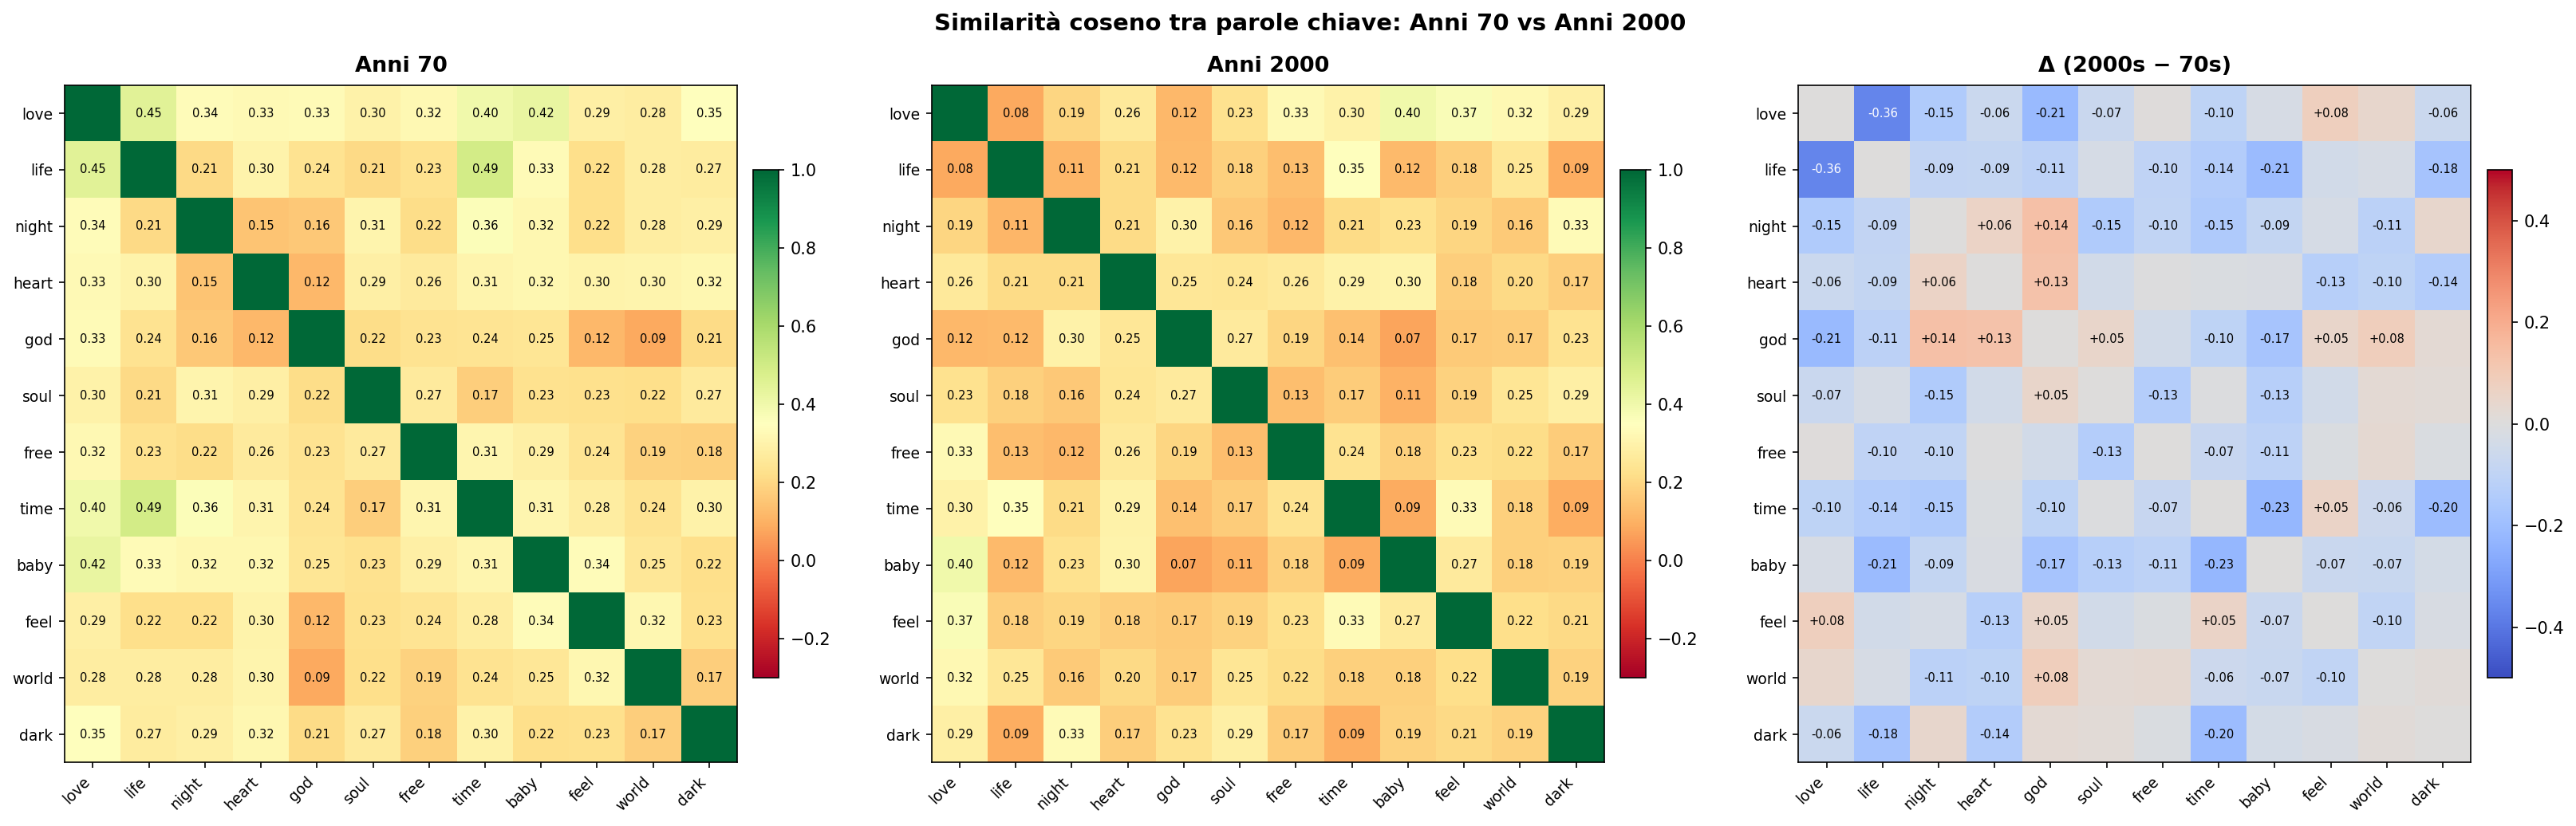
\includegraphics[width=\textwidth]{word2vec_heatmap.png}
\caption{Similarità coseno tra 12 parole chiave: anni 70 (sinistra), anni 2000 (centro), differenza puntuale 2000s$-$70s (destra).}
\label{fig:w2v-heatmap}
\end{figure}

Il pannello di destra rende visibile a colpo d'occhio dove il confronto a coppie isolate (sopra) generalizza bene e dove no: \textit{life}--\textit{love} cala di $-0.36$ (il calo più marcato dell'intera matrice), mentre \textit{night}--\textit{god} e \textit{heart}--\textit{god} salgono di $+0.14$/$+0.13$. Il quadro complessivo è quello di piccoli spostamenti diffusi in entrambe le direzioni piuttosto che un'unica tendenza dominante (es.\ ``tutto si allontana'' o ``tutto si avvicina''), coerente con l'idea che il lessico condiviso fra le due ere si riorganizzi localmente attorno a singole parole più che spostarsi in blocco.

% ============================================================
\section{Analisi del Vocabolario}
% ============================================================

\begin{pylisting}[title={Confronto dei vocabolari tra le due ere}]
vocab_70s   = set(model_70s.wv.index_to_key)
vocab_2000s = set(model_2000s.wv.index_to_key)

solo_70s   = vocab_70s - vocab_2000s    # parole esclusive anni 70
solo_2000s = vocab_2000s - vocab_70s    # parole esclusive anni 2000
comuni     = vocab_70s & vocab_2000s    # parole condivise

# parole caratteristiche (esclusive + frequenti)
interessanti_70s = sorted(
    [p for p in solo_70s   if freq_70s[p]   > 20],
    key=lambda x: -freq_70s[x]
)
interessanti_2000s = sorted(
    [p for p in solo_2000s if freq_2000s[p] > 20],
    key=lambda x: -freq_2000s[x]
)
\end{pylisting}

L'analisi del vocabolario distingue tre insiemi:
\begin{itemize}
  \item \textbf{Parole esclusive degli anni 70} (frequenza $>20$): \textit{boogie, diddley, whop, aaaahh, mustapha, ahha, gentle, zane, bicycle, pity, lucy, chingaling, hitch, bee, hike, ooooh, honky, rockn, andrew, wooh}.
  \item \textbf{Parole esclusive degli anni 2000} (frequenza $>20$): \textit{superstar, hooker, gangsta, yall, rap, retro, muh, ayo, chocolate, freezer, mom, eheh, gaga, gangstas, presents, artpop, idiot, glam, army, spot}.
  \item \textbf{Parole comuni}: il nucleo lessicale condiviso tra le due ere — temi universali come amore, tempo, vita, notte.
\end{itemize}

Confrontando queste liste con il dataset originale emerge un fatto rilevante per l'interpretazione dell'intero esperimento: molte delle parole ``caratteristiche di un'era'' sono in realtà caratteristiche di un singolo artista, non del periodo nel suo complesso. \textit{Mustapha} e \textit{bicycle} compaiono quasi esclusivamente nei brani dei Queen (\textit{Mustapha}, \textit{Bicycle Race}); \textit{diddley} viene da \textit{Diddley Daddy} dei Rolling Stones (una cover di Bo Diddley); dal lato anni 2000, \textit{gaga}, \textit{artpop} e \textit{retro} sono quasi interamente concentrate nei brani di Lady Gaga (il suo stesso nome usato come ad-lib, più il titolo dell'album \textit{Artpop}), e \textit{gangsta} viene esclusivamente da Eminem. Il ``vocabolario esclusivo di un'era'' misura quindi in parte lo stile idiosincratico di un singolo artista molto rappresentato nel campione, non un tratto condiviso del periodo — un limite di selezione degli artisti discusso più a fondo in Sezione~11.5.

% ============================================================
\section{Analisi Sistematica del Semantic Shift}
% ============================================================

\subsection{Coppie con maggiore variazione di similarità}
\label{sec:shift-sistematico}

\begin{pylisting}[title={Analisi sistematica delle coppie di parole comuni (versione vettorizzata)}]
FREQ_COPPIE = 100   # frequenza minima in entrambe le ere

candidati = [
    p for p in (vocab_70s & vocab_2000s)
    if freq_70s[p] >= FREQ_COPPIE and freq_2000s[p] >= FREQ_COPPIE
]

# similarita' vettorizzata: una matrice N x N invece di N^2/2 chiamate a
# .similarity(), utile quando i candidati salgono a qualche centinaio
def matrice_coseno(model, parole):
    vettori = np.array([model.wv[p] for p in parole])
    norme   = vettori / np.linalg.norm(vettori, axis=1, keepdims=True)
    return norme @ norme.T

sim70, sim2000 = matrice_coseno(model_70s, candidati), matrice_coseno(model_2000s, candidati)

coppie_sist = []
for i, w1 in enumerate(candidati):
    for j in range(i + 1, len(candidati)):
        w2, s70, s2000 = candidati[j], float(sim70[i, j]), float(sim2000[i, j])
        coppie_sist.append({
            'w1': w1, 'w2': w2, 's70': s70, 's2000': s2000,
            'delta': abs(s70 - s2000), 'direzione': s2000 - s70,
        })

coppie_sist.sort(key=lambda x: -x['delta'])
\end{pylisting}

Per ogni coppia di parole che compaiono con frequenza sufficiente in \textit{entrambi} i corpus, si calcola il \textbf{delta di similarità}:
\[
  \Delta(w_1, w_2) = |\text{sim}_{70}(w_1, w_2) - \text{sim}_{2000}(w_1, w_2)|
\]

Le coppie con $\Delta$ alto sono quelle la cui relazione semantica è più cambiata tra le due ere. La \textit{direzione} del cambiamento ($\text{sim}_{2000} - \text{sim}_{70}$) indica se le parole si sono avvicinate o allontanate:
\begin{itemize}
  \item \textbf{Direzione positiva}: le due parole sono diventate più associate negli anni 2000.
  \item \textbf{Direzione negativa}: le due parole erano più associate negli anni 70 e si sono semanticamente allontanate.
\end{itemize}

Con soglia \texttt{FREQ\_COPPIE=100} si ottengono \textbf{245 parole candidate} e quindi \textbf{29\,890 coppie} confrontate. Le 5 coppie con delta più alto sono:

\begin{table}[H]
  \centering
  \caption{Top 5 coppie con maggiore variazione di similarità (risultati reali)}
  \small
  \begin{tabular}{lrrrl}
    \toprule
    \textbf{Coppia} & \textbf{Anni 70} & \textbf{Anni 2000} & \textbf{$\Delta$} & \textbf{Trend} \\
    \midrule
    (tell, world)     & 0.447  & 0.000    & 0.447 & più lontane \\
    (fight, two)      & $-0.078$ & 0.332  & 0.409 & più vicine \\
    (remember, lies)  & 0.424  & 0.016    & 0.408 & più lontane \\
    (happy, show)     & 0.428  & 0.022    & 0.406 & più lontane \\
    (old, city)       & $-0.094$ & 0.305  & 0.399 & più vicine \\
    \bottomrule
  \end{tabular}
\end{table}

All'estremo opposto della classifica, le coppie con $\Delta$ più basso mostrano un valore identico fino alla quarta cifra decimale in entrambe le ere:

\begin{table}[H]
  \centering
  \caption{Le 5 coppie con variazione di similarità più bassa (risultati reali)}
  \small
  \begin{tabular}{lrrr}
    \toprule
    \textbf{Coppia} & \textbf{Anni 70} & \textbf{Anni 2000} & \textbf{$\Delta$} \\
    \midrule
    (round, last)       & 0.1493  & 0.1493  & 0.0000 \\
    (watch, run)        & 0.2164  & 0.2164  & 0.0000 \\
    (everyone, stars)   & 0.0607  & 0.0607  & 0.0000 \\
    (gone, lose)        & 0.1860  & 0.1860  & 0.0000 \\
    (bring, sky)        & 0.1347  & 0.1347  & 0.0000 \\
    \bottomrule
  \end{tabular}
\end{table}

\textbf{Attenzione}: questi valori non sono una prova di stabilità semantica genuina fra le due ere. Con $29\,890$ coppie confrontate e i delta distribuiti su un range di poco più di $0.4$, la spaziatura attesa fra valori adiacenti nella distribuzione ordinata è dell'ordine di $10^{-5}$: a questa risoluzione, un certo numero di coppie ottiene un delta praticamente nullo per semplice densità statistica della coda della distribuzione, non perché la relazione fra le due parole sia rimasta davvero identica nei due modelli indipendenti. Va quindi letta come un artefatto dell'ordinamento, non come un risultato interpretabile parola per parola — a differenza delle coppie in testa alla classifica (Tabella~4), il cui $\Delta$ è abbastanza grande da non poter essere spiegato dalla sola densità dei dati.

\subsection{Parole con maggiore cambiamento di contesto}
\label{sec:vocab-shift}

\begin{pylisting}[title={Overlap dei vicini per misurare il semantic shift}]
FREQ_MINIMA  = 30
TOP_N_VICINI = 10

parole_frequenti_comuni = [
    p for p in comuni
    if freq_70s[p] >= FREQ_MINIMA and freq_2000s[p] >= FREQ_MINIMA
]

risultati = []
for parola in parole_frequenti_comuni:
    vicini_70s   = set(w for w,_ in
                   model_70s.wv.most_similar(parola, topn=TOP_N_VICINI))
    vicini_2000s = set(w for w,_ in
                   model_2000s.wv.most_similar(parola, topn=TOP_N_VICINI))

    overlap     = len(vicini_70s & vicini_2000s) / TOP_N_VICINI
    cambiamento = 1 - overlap

    risultati.append({
        'parola': parola, 'cambiamento': cambiamento,
        'overlap': overlap,
        'vicini_70s': vicini_70s, 'vicini_2000s': vicini_2000s,
    })

risultati.sort(key=lambda x: -x['cambiamento'])
\end{pylisting}

L'analisi sistematica calcola, per ogni parola comune frequente, l'overlap tra i 10 vicini più prossimi nelle due ere. Per ciascuna parola nel top-10 si analizza in dettaglio:
\begin{itemize}
  \item I \textbf{vicini spariti}: parole vicine negli anni 70 che non compaiono più nel vicinato degli anni 2000 — indicano contesti culturali scomparsi.
  \item I \textbf{vicini nuovi}: parole vicine negli anni 2000 ma non negli anni 70 — indicano nuovi usi o associazioni culturali.
  \item I \textbf{vicini stabili}: parole rimaste nel vicinato in entrambe le ere — il nucleo semantico stabile della parola.
\end{itemize}

Con soglia \texttt{FREQ\_MINIMA=30} si ottengono \textbf{648 parole comuni} analizzate. Un risultato inatteso: per la maggior parte delle parole nel top-30 (es.\ \textit{dreaming}, \textit{making}, \textit{war}, \textit{follow}, \textit{open}) l'overlap è \textbf{0\%} (cambiamento 100\%) — nessuno dei 10 vicini più prossimi coincide fra le due ere. Questo conferma quanto osservato in Sezione~\ref{sec:parole-simili}: con corpus di poche migliaia di canzoni per era, il vicinato immediato di una parola è dominato da rumore statistico più che da un segnale semantico stabile, e va quindi interpretato con cautela.

Le parole più \textbf{stabili} (overlap più alto, comunque solo 10--30\%) sono \textit{new} (vicini comuni: \textit{brand, orleans, york}), \textit{rest} (\textit{test, vagabonds}), \textit{room} (\textit{hotel}), \textit{roll} (\textit{rock}), \textit{took} (\textit{advantage}), \textit{clothes} (\textit{wear}), \textit{every} (\textit{single}) e \textit{pull} (\textit{plug}). Guardando questi esempi da vicino emerge un pattern linguistico più interessante della semplice ``stabilità'': ciò che sopravvive intatto per 30 anni non sono temi o significati, ma \textbf{collocazioni e formule fisse della lingua} — \textit{brand new}, \textit{New York}, \textit{New Orleans}, \textit{rock and roll}, \textit{hotel room}, \textit{took advantage}, \textit{pull the plug}, \textit{every single}. Il nucleo lessicale che il modello riconosce come invariato nel tempo è quindi prevalentemente \textbf{collocazionale}, non semantico: espressioni multi-parola così frequenti e rigide da restare ancorate le une alle altre indipendentemente dall'era, mentre il resto del vocabolario si muove liberamente.

La Figura~\ref{fig:w2v-drift} visualizza insieme i due risultati di questa sezione: a sinistra le top-20 parole per grado di cambiamento (Sezione~\ref{sec:vocab-shift}), quasi tutte al 100\%; a destra lo scatter delle $29\,890$ coppie confrontate in Sezione~\ref{sec:shift-sistematico}, con le coppie a delta più alto (fra cui \textit{tell--world} e \textit{happy--show}) annotate esplicitamente.

\begin{figure}[H]
\centering
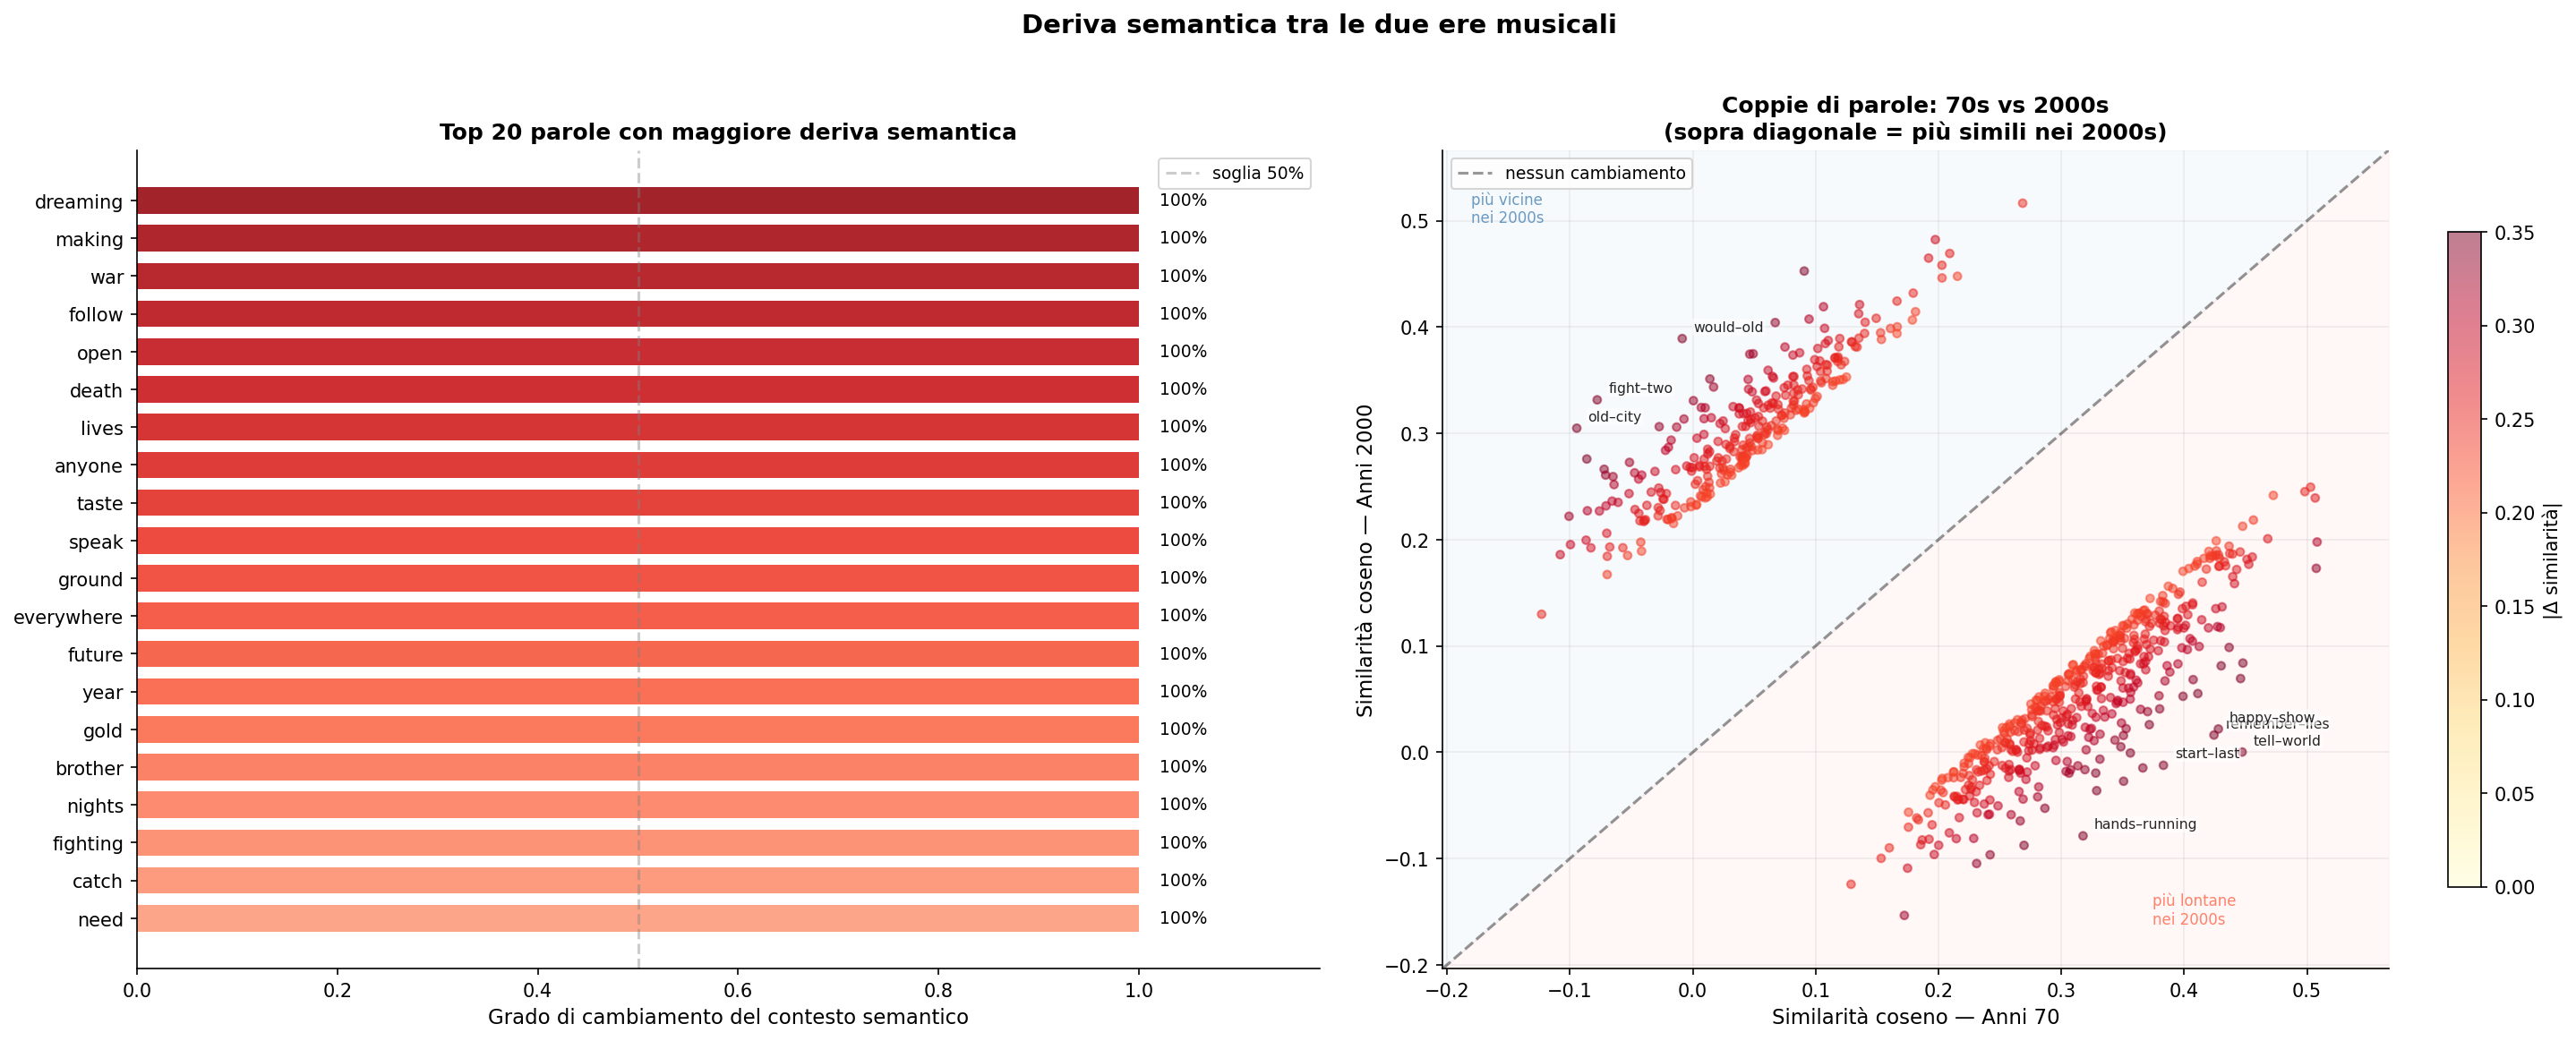
\includegraphics[width=\textwidth]{word2vec_drift.png}
\caption{Deriva semantica: (sinistra) top-20 parole per grado di cambiamento di contesto; (destra) similarità coseno delle coppie di parole comuni, anni 70 vs anni 2000 — sopra la diagonale indica coppie diventate più simili nei 2000s, sotto indica coppie diventate più distanti.}
\label{fig:w2v-drift}
\end{figure}

Lo scatter a destra rende visibile un aspetto che le sole tabelle non mostrano: la nuvola di punti è nettamente sbilanciata sotto la diagonale, cioè la maggioranza delle coppie comuni risulta \emph{meno} simile nel 2000 che negli anni 70, non semplicemente ``diversa in modo casuale''. Questo è coerente con un vocabolario condiviso che, negli anni 2000, viene ricombinato in configurazioni sintattiche/collocazionali più varie (si veda anche la lettura dei cluster in Sezione~9) piuttosto che con un lessico comune che resta stabile nel tempo.

% ============================================================
\section{Clustering K-Means}
% ============================================================

\begin{pylisting}[title={Clustering K-Means sulle top 200 parole}]
def fai_clustering(model, n_clusters=6, top_words=200):
    parole  = model.wv.index_to_key[:top_words]   # top 200 per freq
    vettori = np.array([model.wv[w] for w in parole])
    # normalizza a norma unitaria: senza, un vettore con norma anomala
    # domina la distanza euclidea di K-Means e resta isolato in un cluster singoletto
    vettori_norm = vettori / np.linalg.norm(vettori, axis=1, keepdims=True)
    km      = KMeans(n_clusters=n_clusters, random_state=42, n_init=10)
    labels  = km.fit_predict(vettori_norm)
    cluster = {}
    for p, l in zip(parole, labels):
        cluster.setdefault(l, []).append(p)
    return cluster, list(parole), vettori, labels

cl_70s,   par_70s,   vec_70s,   lbl_70s   = fai_clustering(model_70s)
cl_2000s, par_2000s, vec_2000s, lbl_2000s = fai_clustering(model_2000s)
\end{pylisting}

Il clustering opera sulle \textbf{200 parole più frequenti} del vocabolario di ciascun modello, raggruppandole in $k=6$ cluster tramite K-Means applicato ai vettori Word2Vec a 100 dimensioni.

\begin{table}[H]
  \centering
  \caption{Cluster K-Means, anni 70 (risultati reali, prime 12 parole per cluster)}
  \small
  \begin{tabular}{c>{\raggedright\arraybackslash}p{11.5cm}}
    \toprule
    \textbf{Cluster} & \textbf{Parole} \\
    \midrule
    0 & love, got, baby, yeah, want, well, take, gonna, away, let, make, right \\
    1 & get, come, man, back, tell, home, find, woman, better, people, dance, old \\
    2 & feel, heart, world, long, good, still, said, ooh, keep, gone, hey, alone \\
    3 & say, would, going, always, turn, nothing, end, dream, everything, must, call, someone \\
    4 & know, see, little, look, think, girl, light, please, bad, thing, put, blue \\
    5 & like, time, one, never, way, life, night, could, day, eyes, give, every \\
    \bottomrule
  \end{tabular}
\end{table}

\begin{table}[H]
  \centering
  \caption{Cluster K-Means, anni 2000 (risultati reali, prime 12 parole per cluster)}
  \small
  \begin{tabular}{c>{\raggedright\arraybackslash}p{11.5cm}}
    \toprule
    \textbf{Cluster} & \textbf{Parole} \\
    \midrule
    0 & got, time, away, around, need, life, night, day, mind, gone, thing, face \\
    1 & love, one, want, never, way, take, feel, right, little, every, everything, always \\
    2 & like, know, get, yeah, come, cause, baby, make, give, think, eyes, ooh \\
    3 & let, world, girl, hold, stop, going, show, wrong, live, dance, beautiful, far \\
    4 & back, well, heart, look, find, nothing, tonight, last, put, head, better, turn \\
    5 & see, say, gonna, could, wanna, said, home, man, still, would, even, alone \\
    \bottomrule
  \end{tabular}
\end{table}

Dopo aver normalizzato i vettori a norma unitaria prima del clustering (un vettore con norma anomala, in K-Means con distanza euclidea, finiva isolato in un cluster singoletto — un artefatto risolto rendendo la geometria del clustering coerente con la cosine similarity usata nel resto dell'analisi), i sei cluster risultano ben bilanciati per entrambe le ere. Lavorando sulle 200 parole più \textbf{frequenti} (non su un campione casuale del vocabolario), restano comunque dominati da parole funzionali e verbi comuni (\textit{know, got, get, come}) piuttosto che da lessico tematico raro: il risultato è quindi più vicino a una segmentazione \textbf{sintattico-collocazionale} che a una netta separazione per macrotema. Alcuni cluster sono comunque interpretabili, e soprattutto \textbf{ricorrono in entrambe le ere}: il cluster 0 degli anni 70 (\textit{love, baby, want, gonna, away, make, right}) e il cluster 1 degli anni 2000 (\textit{love, want, feel, right, everything, always}) condividono lo stesso registro di desiderio/relazione affettiva; il cluster 5 degli anni 70 (\textit{time, life, night, day, eyes}) e il cluster 0 degli anni 2000 (\textit{time, life, night, day, mind, face}) condividono un registro temporale/esistenziale simile. Più che rivelare macrotemi distinti per epoca, il clustering mostra quindi una struttura sintattico-tematica di fondo piuttosto stabile nel tempo. Va comunque ribadito il limite già discusso in Sezione~\ref{sec:parole-simili}: con corpus di questa dimensione le strutture emergenti vanno lette come indicazioni, non come conclusioni robuste.

% ============================================================
\section{Visualizzazione t-SNE}
% ============================================================

\begin{pylisting}[title={Riduzione dimensionale t-SNE e plot dei cluster}]
def tsne_plot(parole, vettori, labels, titolo, ax, n_clusters=6):
    # niente max_iter/n_iter esplicito: il nome cambia tra versioni di
    # scikit-learn, il default (1000) e' comunque quello voluto
    tsne = TSNE(n_components=2, random_state=42, perplexity=30)
    v2d  = tsne.fit_transform(vettori)  # 100D -> 2D

    colori    = plt.cm.Set1(np.linspace(0, 1, n_clusters))
    highlight = {
        'love', 'night', 'heart', 'baby', 'time',
        'world', 'life', 'feel', 'fire', 'rain',
        'sun', 'soul', 'free', 'dark', 'light', 'god'
    }

    for cid in range(n_clusters):
        mask = labels == cid
        ax.scatter(v2d[mask, 0], v2d[mask, 1],
                   c=[colori[cid]], label=f'Cluster {cid}',
                   alpha=0.7, s=60)

    # annota le parole semanticamente rilevanti
    for i, p in enumerate(parole):
        if p in highlight:
            ax.annotate(p, (v2d[i, 0], v2d[i, 1]),
                        fontsize=9, fontweight='bold',
                        xytext=(5, 5), textcoords='offset points')
\end{pylisting}

Il grafico t-SNE mostra la distribuzione delle 200 parole più frequenti in 2D, con colori diversi per cluster. Le parole semanticamente rilevanti (amore, vita, notte, cuore, ecc.) vengono annotate direttamente sul grafico per facilitare l'interpretazione.

\begin{figure}[H]
\centering
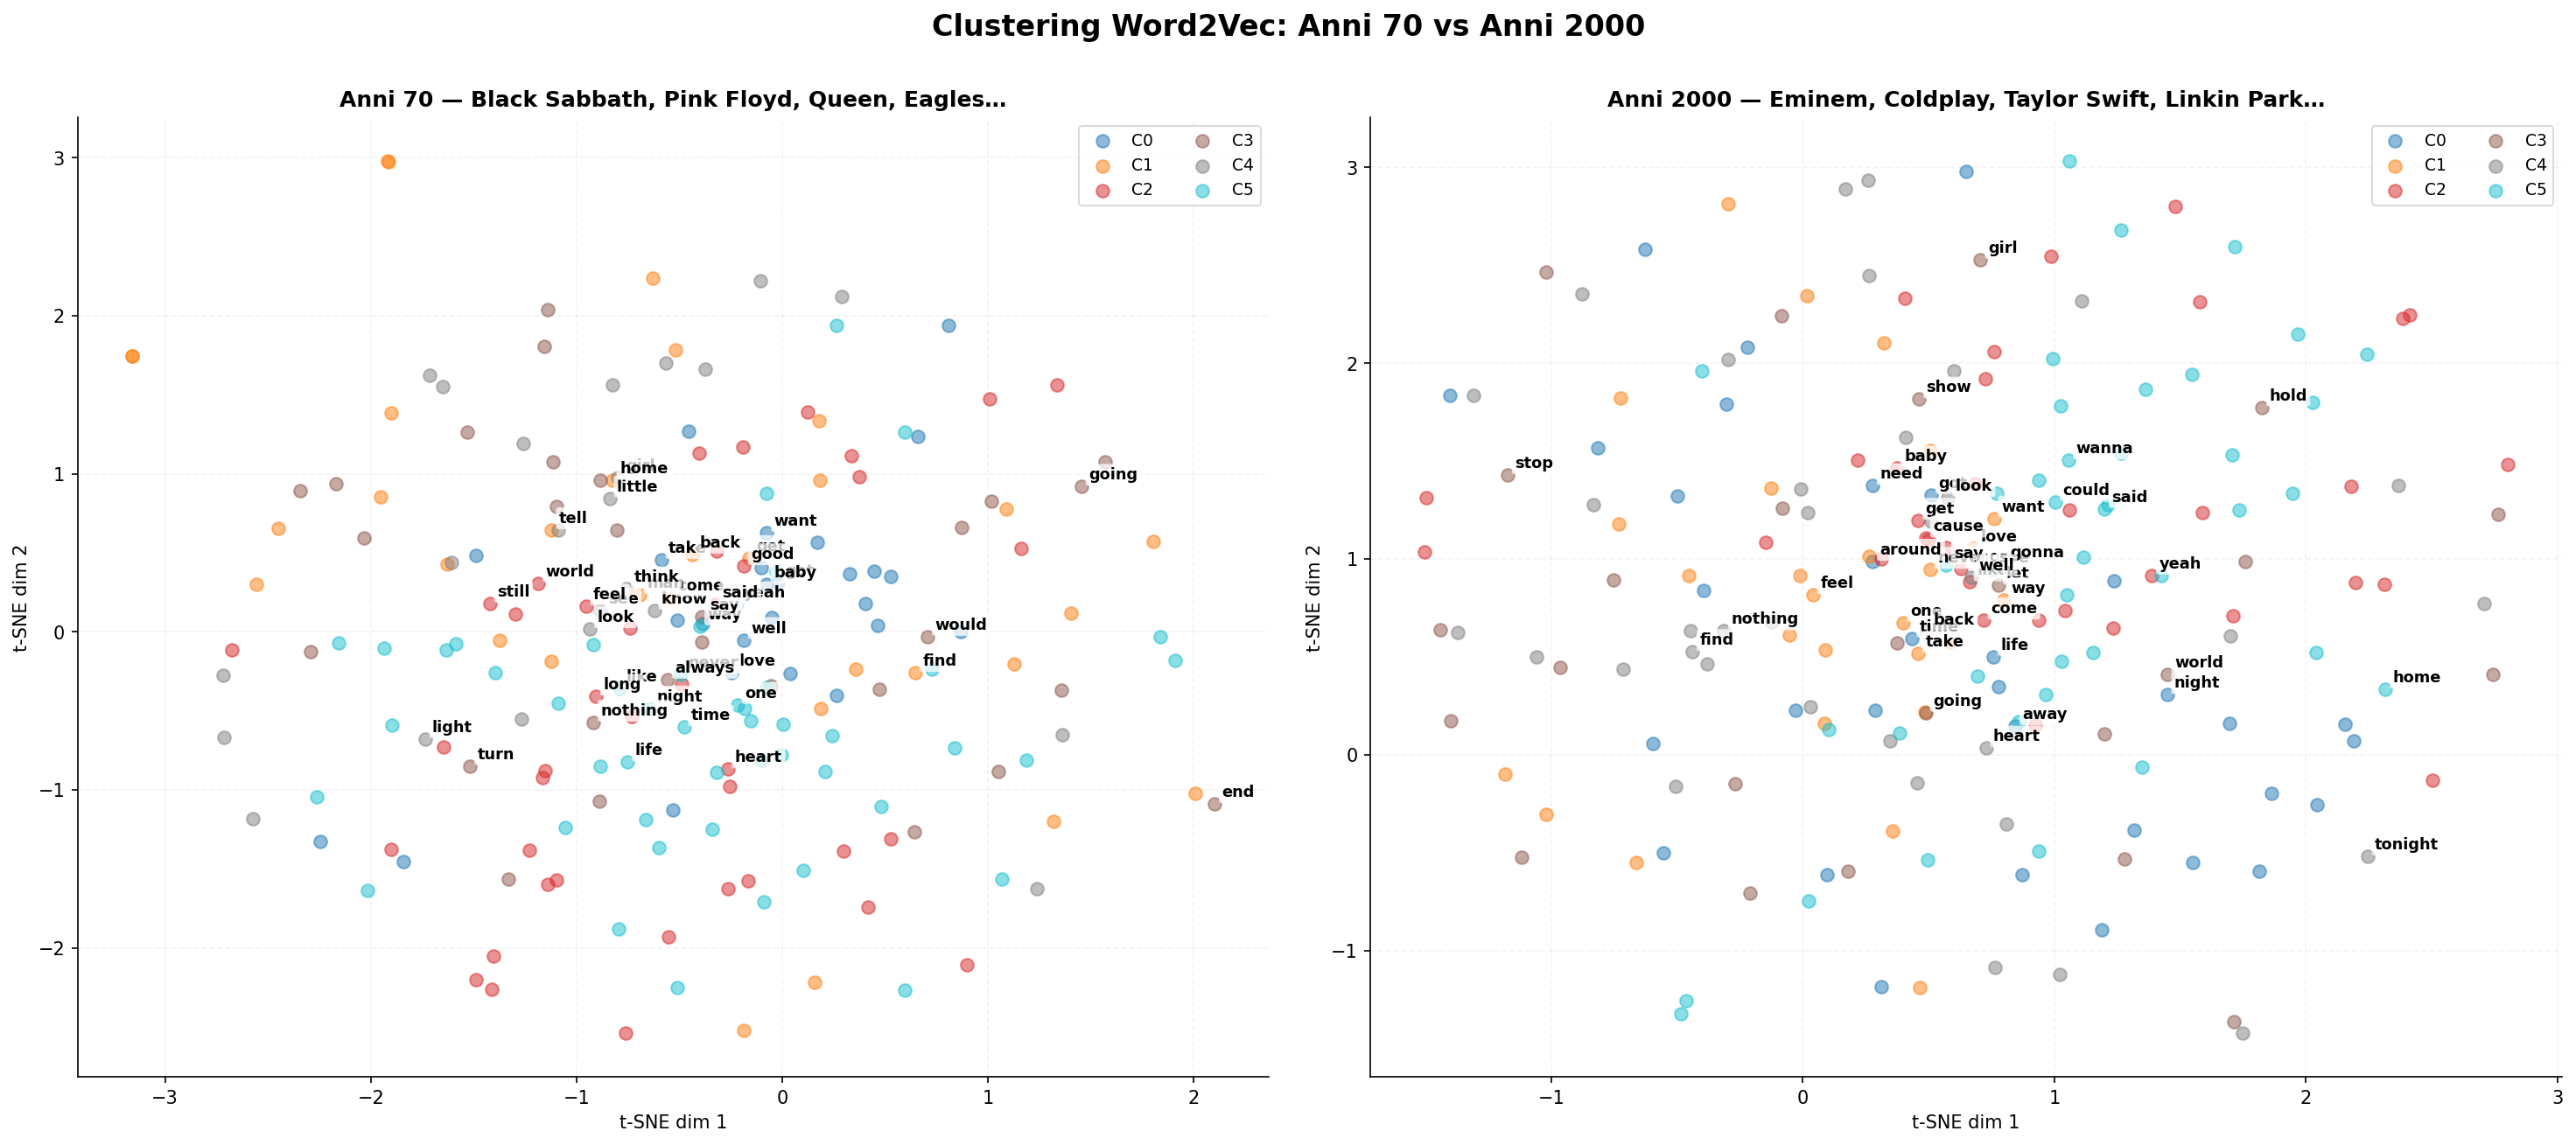
\includegraphics[width=\textwidth]{word2vec_cluster.png}
\caption{Proiezione t-SNE dei 6 cluster K-Means, anni 70 (sinistra) vs anni 2000 (destra), con le parole tematicamente rilevanti annotate.}
\label{fig:w2v-tsne}
\end{figure}

La disposizione dei punti rivela la \textbf{struttura interna} del lessico di ciascuna era: se i cluster sono ben separati, il linguaggio è più specializzato per tema; se i cluster si sovrappongono, il lessico è più polisemico e interdipendente. In entrambe le proiezioni i cluster appaiono visivamente sovrapposti, senza una separazione netta in regioni distinte del piano — coerente con la lettura data in Sezione~9: sulle 200 parole più frequenti il segnale dominante è collocazionale/sintattico, non tematico, e t-SNE (che preserva la struttura locale ma non necessariamente crea macro-isole ben separate) rende visivamente evidente proprio questa continuità, più che una netta suddivisione in macrotemi.

% ============================================================
\section{Risultati e Discussione}
% ============================================================

\subsection{Il paradosso della scala: esempi singoli rumorosi, statistiche aggregate più robuste}

Le due ere condividono \textbf{2973 parole} sulle rispettive 4752 (anni 70) e 4800 (anni 2000) del vocabolario Word2Vec, con oltre 1700 parole esclusive per lato (Sezione~4). Interrogando questo spazio su singole parole isolate — i vicini di \textit{love} o \textit{night} (Sezione~\ref{sec:parole-simili}), o l'overlap dei vicini per le 648 parole comuni (Sezione~\ref{sec:vocab-shift}) — il segnale è quasi sempre dominato dal rumore: la maggioranza delle parole nel top-30 per cambiamento ha overlap $0\%$. Con corpus di 1729 e 1312 canzoni, ogni parola compare in troppi contesti diversi per stabilizzare un vicinato semantico coerente.

Il quadro cambia passando all'\textbf{analisi aggregata su centinaia di coppie} (Sezione~\ref{sec:shift-sistematico}): filtrando le 245 parole con frequenza $\geq 100$ e confrontando le $29\,890$ coppie possibili, i pattern nella coda della distribuzione risultano più difendibili perché emergono da un confronto sistematico, non da una scelta soggettiva — a patto di scartare le coppie con $\Delta$ quasi nullo, che sono un artefatto di densità statistica più che un segnale di stabilità reale (si veda l'avvertenza in Sezione~\ref{sec:shift-sistematico}). Un risultato più solido di un singolo numero isolato viene invece dal confronto con i vicini più stabili in assoluto (Sezione~\ref{sec:vocab-shift}): non si tratta di temi condivisi, ma di \textbf{collocazioni fisse della lingua} (\textit{brand new}, \textit{rock and roll}, \textit{hotel room}) — il nucleo del lessico musicale che il tempo non cambia è collocazionale, non semantico.

\subsection{Cosa aggiunge il clustering rispetto alle coppie di parole}

Il clustering K-Means (Sezione~9) analizza la struttura del vocabolario da un'angolazione complementare alle coppie: la geometria complessiva delle 200 parole più frequenti. I cluster ottenuti sono prevalentemente \textbf{sintattico-collocazionali} (dominati da verbi e parole funzionali, es.\ \textit{know, got, get, come}) piuttosto che tematici, perché le parole più frequenti sono anche le più polisemiche. Lo stesso tipo di cluster — un nucleo di desiderio/relazione affettiva, uno temporale/esistenziale — ricompare in entrambe le ere con parole in parte diverse, segno che a restare stabile nel tempo è la struttura sintattico-tematica di fondo, più che uno specifico insieme di macrotemi.

\subsection{Sintesi: cosa può (e non può) dimostrare questo esperimento}

Nel complesso, i risultati supportano un'affermazione \textbf{qualitativa} solida — i due corpora occupano regioni lessicali parzialmente sovrapposte ma distinte, coerenti con i generi musicali attesi nelle due ere — ma non affermazioni \textbf{quantitative} forti sul cambiamento semantico di una singola parola, che restano suggestive più che dimostrate. Servirebbero corpus ordini di grandezza più grandi, più artisti per era e un test di significatività statistica, oggi assenti. Resta comunque un risultato metodologicamente utile: mostra dove passa il confine fra ciò che Word2Vec rivela in modo affidabile a piccola scala (statistiche aggregate) e ciò che richiede cautela (giudizi su parole isolate).

\begin{table}[H]
  \centering
  \caption{Riepilogo comparativo delle caratteristiche dei due corpus}
  \begin{tabular}{lrr}
    \toprule
    \textbf{Caratteristica}       & \textbf{Anni 70}       & \textbf{Anni 2000} \\
    \midrule
    Artisti rappresentativi       & 12                     & 11 \\
    Generi principali             & Rock, Glam, Disco      & Pop, Rap, Alt-rock \\
    Canzoni (post-pulizia)        & 1\,729                 & 1\,312 \\
    Token totali                  & 163\,180               & 149\,820 \\
    Token unici (post-pulizia)    & 11\,174                & 11\,551 \\
    Vocabolario Word2Vec          & 4\,752                 & 4\,800 \\
    Parole esclusive              & 1\,779                 & 1\,827 \\
    \bottomrule
  \end{tabular}
  \\[0.3em]
  {\footnotesize Parole comuni ai due vocabolari: 2\,973 (Sezione~4).}
\end{table}

\subsection{Osservazioni principali}

\begin{enumerate}
  \item \textbf{Le rappresentazioni vettoriali riflettono differenze di dominio a livello aggregato}: sulle singole parole isolate (es.\ \textit{love}, \textit{night}) i vicini estratti sono in gran parte rumore (Sezione~\ref{sec:parole-simili}), ma su statistiche aggregate su centinaia di parole il segnale diventa più affidabile (Sezione~11.1).

  \item \textbf{Il semantic shift sistematico è più informativo dell'overlap puntuale}: l'overlap dei 10 vicini più prossimi satura a 0\% per la stragrande maggioranza delle 648 parole comuni analizzate (Sezione~\ref{sec:vocab-shift}), mentre l'analisi aggregata sulle 29\,890 coppie (Sezione~\ref{sec:shift-sistematico}) individua candidati di deriva semantica più difendibili.

  \item \textbf{Il vocabolario esclusivo rivela più il bias di selezione che il periodo storico}: molte parole presenti solo in un'era, verificate contro il dataset originale, si rivelano specifiche di un singolo artista (es.\ \textit{mustapha}, \textit{bicycle} per i Queen; \textit{gaga}, \textit{artpop} per Lady Gaga) più che rappresentative dell'intera era (Sezione~7).

  \item \textbf{I cluster K-Means sono prevalentemente sintattico-collocazionali, non tematici}: lavorando sulle 200 parole più frequenti (le più polisemiche) i gruppi emergono attorno a verbi e parole funzionali comuni, con solo alcune isole tematicamente interpretabili (Sezione~9).

  \item \textbf{t-SNE conferma la sovrapposizione dei cluster}: nelle proiezioni 2D i cluster appaiono visivamente sovrapposti anziché ben separati, coerente con un segnale collocazionale/sintattico piuttosto che una netta suddivisione in macrotemi (Sezione~10).

  \item \textbf{Il nucleo lessicale più stabile nel tempo è collocazionale, non semantico}: le parole con vicinato più invariato fra le due ere non condividono un tema, ma fanno parte di espressioni fisse della lingua (\textit{brand new}, \textit{rock and roll}, \textit{hotel room}, Sezione~\ref{sec:vocab-shift}) — ciò che 30 anni di musica non cambiano sono le formule linguistiche congelate, non i significati.
\end{enumerate}

\subsection{Limiti dell'approccio}

\begin{itemize}
  \item \textbf{Bias nella selezione degli artisti, dimostrato non solo ipotizzato}: la scelta manuale degli artisti introduce un bias soggettivo, ed è verificabile concretamente nei dati (Sezione~7) — parole ``caratteristiche di un'era'' come \textit{mustapha}, \textit{bicycle} (Queen) o \textit{gaga}, \textit{artpop} (Lady Gaga) sono in realtà specifiche di un singolo artista molto rappresentato nel campione. Artisti diversi avrebbero potuto dare risultati differenti.
  \item \textbf{Corpus sbilanciati}: se gli artisti degli anni 2000 hanno in media più canzoni nel dataset, il modello corrispondente sarà addestrato su più dati, rendendo il confronto non del tutto omogeneo.
  \item \textbf{Spazi vettoriali non allineati}: i due modelli sono addestrati indipendentemente; gli spazi vettoriali risultanti non sono direttamente comparabili tramite distanza euclidea — la similarità coseno interna a ciascun modello è però robusta.
  \item \textbf{Dipendenza dal preprocessing}: la rimozione delle stopwords e dei token corti può eliminare parole grammaticalmente significative.
\end{itemize}

% ============================================================
\section{Conclusioni}
% ============================================================

Il laboratorio ha dimostrato come Word2Vec, applicato a testi musicali, sia in grado di catturare differenze semantiche e culturali tra due ere distanti nel tempo. I modelli addestrati separatamente sugli anni 70 e sugli anni 2000 producono spazi vettoriali che riflettono i diversi immaginari, temi e registri linguistici delle rispettive epoche.

L'analisi sistematica del semantic shift — tramite overlap dei vicini e delta di similarità — permette di identificare quantitativamente quali parole hanno cambiato contesto d'uso e in quale direzione, con maggiore affidabilità quando condotta su statistiche aggregate piuttosto che su singole parole isolate. I cluster K-Means e la visualizzazione t-SNE completano l'analisi con una prospettiva strutturale: sulle parole più frequenti la struttura che emerge è prevalentemente sintattico-collocazionale, con solo alcuni nuclei tematici riconoscibili. Il risultato più robusto dell'intera analisi è forse il più controintuitivo: ciò che resta stabile nel lessico musicale a 30 anni di distanza non sono i temi, ma le \textbf{collocazioni fisse} della lingua (\textit{brand new}, \textit{rock and roll}, \textit{hotel room}).

Questo tipo di analisi, applicabile a qualsiasi corpus diacronico, mostra il potenziale delle rappresentazioni distribuzionali per lo studio dell'evoluzione del linguaggio nel tempo.

% ============================================================
\section{Dichiarazione sui Contributi di IA}
% ============================================================

Per questo laboratorio ci siamo appoggiati anche a uno strumento di intelligenza artificiale generativa (Claude, Anthropic), usato come supporto puntuale durante lo sviluppo e non come autore del lavoro. Qualche esempio concreto di come lo abbiamo usato:

\begin{itemize}
  \item \textbf{Correzione di un bug metodologico (Skip-gram vs.\ CBOW)}: il codice non impostava esplicitamente \texttt{sg=1}, quindi Gensim addestrava silenziosamente un modello CBOW nonostante testo e relazione dichiarassero Skip-gram; corretto impostando il parametro esplicitamente (Sezione~2.2).
  \item \textbf{Verifica dei dati contro il dataset reale}: \textit{Led Zeppelin}, incluso nella selezione iniziale degli artisti anni 70, non è risultato presente nel dataset con questo nome esatto — un fallimento silenzioso di \texttt{df['artist'].isin(...)} che sarebbe passato inosservato. Sostituito con \textit{Black Sabbath} e aggiunto un controllo esplicito sul numero di artisti effettivamente trovati (Sezione~3.2).
  \item \textbf{Vettorizzazione del calcolo di similarità}: l'analisi sistematica delle coppie di parole (Sezione~\ref{sec:shift-sistematico}, 245 parole, quasi 30\,000 coppie) usava $O(N^2)$ chiamate a \texttt{.similarity()}; sostituito con un unico prodotto matriciale, necessario per rendere l'analisi eseguibile in tempi ragionevoli.
  \item \textbf{Correzione della pipeline di pulizia}: le contrazioni inglesi (\textit{don't}, \textit{you're}) perdevano l'apostrofo prima del filtro stopword, restando nel corpus come rumore lessicale; aggiunte esplicitamente le forme contratte più comuni alla lista di stopword (Sezione~3.3).
  \item \textbf{Discussione sui limiti dell'analisi}: confronto sui limiti metodologici del confronto tra i due modelli (bias nella selezione manuale degli artisti, corpus di dimensioni sbilanciate, spazi vettoriali non allineati fra le due ere) — si veda Sezione~11.5.
  \item \textbf{Organizzazione dell'output a console}: le stampe dei risultati (tabelle di parole simili, coppie di similarità, deriva semantica) sono state riformattate con colonne allineate e separatori (es.\ \texttt{\{:<12\}}, \texttt{\{:>8.4f\}}), per rendere l'output leggibile durante l'esecuzione invece di semplici \texttt{print} non allineati.
  \item \textbf{Correzione della riproducibilità e di un clustering degenere}: con \texttt{workers=4} il training di Gensim non è bit-esatto a parità di seed, e un run diverso da quello usato per compilare la relazione produceva numeri diversi in tutte le tabelle. Corretto impostando \texttt{workers=1} (costo trascurabile su questo corpus) e rigenerando l'intera relazione da un unico run congelato. Nello stesso passaggio si è notato che il clustering K-Means produceva occasionalmente cluster singoletto: risolto normalizzando i vettori a norma unitaria prima di applicare K-Means, coerentemente con la cosine similarity usata nel resto dell'analisi.
\end{itemize}

L'impostazione del lavoro, le scelte metodologiche, l'interpretazione critica dei risultati e la stesura della relazione restano nostre.

\end{document}
